\documentclass[sn-mathphys-num]{sn-jnl}% Math and Physical Sciences Numbered Reference Style 

\usepackage{graphicx}%
\usepackage{multirow}%
\usepackage{amsmath,amssymb,amsfonts}%
\usepackage{amsthm}%
\usepackage{mathrsfs}%
\usepackage[title]{appendix}%
\usepackage{xcolor}%
\usepackage{textcomp}%
\usepackage{manyfoot}%
\usepackage{booktabs}%
\usepackage{algorithm}%
\usepackage{algorithmicx}%
\usepackage{algpseudocode}%
\usepackage{listings}%

%% as per the requirement new theorem styles can be included as shown below
\theoremstyle{thmstyleone}%
\newtheorem{theorem}{Theorem}%  meant for continuous numbers
\newtheorem{proposition}[theorem]{Proposition}% 

\theoremstyle{thmstyletwo}%
\newtheorem{example}{Example}%
\newtheorem{remark}{Remark}%

\theoremstyle{thmstylethree}%
\newtheorem{definition}{Definition}%

\raggedbottom
%%\unnumbered% uncomment this for unnumbered level heads

\begin{document}

\title[Article Title]{Air pollution study over decade in Indonesia}

\author[1]{\fnm{Aksamala} \sur{Arfendi}}
\author[1]{\fnm{Eny} \sur{Latifah}}
\author*[1]{\fnm{Hafizh} \sur{Prihtiadi}}\email{hafizhp.fmipa@um.ac.id}

\affil*[1]{\orgdiv{Department of Physics}, \orgname{Universitas Negeri Malang}, \city{Malang}, \postcode{65145}, \state{Malang}, \country{Indonesia}}

\abstract{Air pollution and climate change are general problems for society. This paper proposes an integrated analysis of the Air Quality Index (AQI) and meteorological conditions over Indonesia. The column-based data integration model is applied to create integrated data of the Air Quaility Index and meteorological conditions. The integrated data is then used to generate a causal graph using the PC algorithm. The causal graph reveals that there exist casual relationships between pollutants and meteorological conditions, e.g, humidity, rainfall, wind speed, and duration of sunshine affect particulate matter 10 (PM$_{10}$), wind speed affects sulfur dioxide SO$_{2}$; temperature affects ozone (O$_{3}$). The historical data records that the average wind speed is decreased and the nubre of unhealthy days has risen. Ozone and particulate matter are two pollutants that mainly influence poor air quality in Jakarta. The integrated data is also used to train Long Short-Term Memory (LSTM) and Gated Recurrent Unit (GRU) for forecasting. Experimental results show that LSTM using integrated data produces smaller errors for forecasting AQI and meteorological conditions. (Paper Jakarta)

The results showed that
highlighting this study's importance in supporting strategic planning and providing an early warning system to reduce outdoor activity during extreme pollution.

Datanya CO, NO2, PM2, SO

Air pollution has emerged as a critical environmental challenge with significant implications for public health, economic productivity, and sustainable development across the Indonesian archipelago. Major atmospheric pollutants, including nitrogen oxides (NO$_2$), carbon monoxide (CO), sulfur dioxide (SO$_2$), and fine particulate matter (PM$_{2.5}$), are key contributors to degraded air quality and elevated Air Quality Index (AQI) levels. Exposure to these pollutants has been strongly associated with respiratory diseases, cardiovascular disorders, and increased premature mortality, placing a substantial burden on public health systems. In addition to health impacts, poor air quality also generates significant economic losses through increased healthcare expenditures, reduced labor productivity, disruption of transportation and aviation, and decreased tourism activity. These challenges are particularly pronounced in Indonesia due to rapid urbanization, industrial activities, transportation emissions, and recurrent biomass burning events that frequently affect large parts of the region. Furthermore, the complex atmospheric dynamics of the Maritime Continent—characterized by monsoonal circulation, strong convection, and regional-scale transport of pollutants—create highly variable spatiotemporal pollution patterns. Understanding the behavior, variability, and drivers of key pollutants such as NO$_2$, CO, SO$_2$, and PM$_{2.5}$ is therefore essential for improving air quality management, supporting evidence-based environmental policy, and mitigating the socioeconomic and health impacts of air pollution across Indonesia. Machine learning approaches provide an effective framework for identifying complex nonlinear relationships among pollutants and meteorological variables, enabling more accurate assessment and prediction of AQI variability over the region.

}

\keywords{air pollution, machine learning, GHE,}


\maketitle
\section{Introduction}\label{sec1}
Latar belakang sejarahnya, ML, 

	The World Health Organization (WHO) estimates that approximately 7 million deaths worldwide each year are attributable to air pollution \cite{WorldHealthOrganization2024}. In Indonesia, air pollution is estimated to reduce average life expectancy by about 1.2 years, resulting in an estimated total loss of 309 million life-years due to air pollution \cite{Madrigano2024}. The transportation sector is identified as the primary source of air pollution; according to the European Environment Agency (EEA), transportation activities contribute approximately $56{,}5\%$ of total air pollutant emissions \cite{EEA2022Transport}. Moreover, the rapid growth in motor vehicle ownership has exacerbated emission levels, with the number of registered motor vehicles in Indonesia reaching 146.8 million units in 2018 and exhibiting an average annual growth rate of $8{,}3\%$ \cite{Dimension2022}.
	Particulate matter with a diameter of $\leq 2.5,\mu\text{m}$ (\textit{PM}${2.5}$) is one of the major forms of air pollution that poses serious risks to human health. \textit{PM}${2.5}$ consists of {\itshape primary} and {\itshape secondary} particles, the latter being formed through chemical reactions in the atmosphere, and is commonly associated with various gaseous pollutants such as {\itshape carbon monoxide} (CO), {\itshape nitrogen dioxide} (NO$_2$), and {\itshape sulfur dioxide} (SO$2$). The concentration of \textit{PM}${2.5}$ is considered to be at an unhealthy level when it exceeds air quality threshold values, namely above 55.5~$\mu$g/m$^3$ according to the Indonesian Air Pollution Standard Index (ISPU), or above 15~$\mu$g/m$^3$ based on the World Health Organization (WHO) air quality guidelines.
	The Indonesian Agency for Meteorology, Climatology, and Geophysics (BMKG) reported that in 2024, air quality and meteorological conditions in Indonesia exhibited a strong interconnection. Elevated concentrations of greenhouse gases (CO$_2$, CH$_4$, and N$_2$O) contributed to an increase in the national mean surface temperature of up to $0.8^{\circ}\mathrm{C}$, making 2024 the warmest year on record. These conditions were also associated with the occurrence of acid rain, with observed rainfall pH values ranging from 4.33 to 6.53 across multiple regions \cite{BidangKlimatologiBadanMeteorologi2024}.
	Many studies have adopted ML models for Air Pollution Standard prediction across various urban regions, leveraging multiple pollutants and meteorological parameters.
	This study was conducted to examine the relationship between air pollutants and meteorological conditions in Indonesia. The main issue in this study is how to analyze the relationship between surface-level air pollution and meteorological conditions in Indonesia. This article proposes an integrated analysis between the Air Quality Index (AQI) and meteorological conditions using a machine learning approach, integrating surface air pollutant concentrations to capture the dynamic interaction between air quality and atmospheric variability. This article applies the Long Short-Term Memory (LSTM) and Gated Recurrent Unit (GRU) methods to predict AQI values and meteorological variables. The main contribution of this research is the development of an integration framework to analyze the interdependence between variables and to predict future AQI values and meteorological conditions, with a case study in Indonesia.
	The historical data of Air Quality Index (AQI) and meteorological conditions in Jakarta record some important information. The increasing number of unhealthy days happened from 2010-2013, 2015-2018, and 2020-2021. It is understandable that in 2020, the air quality was getting better because of the limited activities during the Covid-19 outbreak. However, the number of unhealthy days raised in 2021. From 2010 to 2021 the number of unhealthy days is always higher that healthy days. This is an early warning for the society that poor air quality might worsen if it is not managed properly. The average temperature slightly increased around 0.55$^\circ$ from 2013 to 2019 and the average wind speed decreased.

Satellite
TROPOMI provides global daily coverage in continuous 5.5 $\times$ km$^{2}$ (nadir) pixels, increasing the data density relative to GOSAT by more than 2 orders of magnitude through the use of an imaging grating spectrometer. It measures in the 2.3 $\mu$m band, where the CO$_{2}$ proxy approach is not possible, with a spectral resolution of 0.25 nm. Retrieval of XCH$_{4}$ by TROPOMI employs a full-physics approach in which surface albedo and atmospheric scattering properties are retrieved to gether with XCH$_{4}$, utilizing additional information from the near-infrared (NIR) band to TROPOMI

We considered two candidates ML methods (Gated Recurrent Unit and Long Short-Term Memory) that rely on ensembles of decision trees (Kingsford, 2008-01). 

Machine learning (ML) algorithm have recently introduced as innovative developments in the bottom-up approaches to upscale data-driven in-situ models to spatially explicit gridded estimates. (paper thailand).

Research Gap - Despite increasing concerns about air pollution in Indonesia, comprehensive studies on Air Quality Index (AQI) dynamics across the Indonesian archipelago remain limited. Most previous research has focused on localized urban air quality assessments, particularly in major cities such as Jakarta and Surabaya, and often relies primarily on ground-based monitoring stations. However, the spatial coverage of monitoring networks across Indonesia is still sparse and uneven, especially over remote islands and rural regions. Furthermore, conventional statistical approaches used in many studies may not adequately capture the complex nonlinear interactions between atmospheric pollutants and meteorological factors. Although machine learning methods have been widely applied in air quality studies in North America, Europe, and East Asia, their application in Indonesia remains relatively scarce, particularly in studies integrating multiple pollutant species such as NO$_2$, CO, SO$_2$, and PM$_{2.5}$ with large-scale atmospheric datasets. As a result, there is still a significant knowledge gap in understanding the large-scale spatiotemporal variability and predictive behavior of air pollution across the Indonesian Maritime Continent.

Research Novelty - This study aims to address these limitations by integrating atmospheric reanalysis data from ERA5 produced by the European Centre for Medium-Range Weather Forecasts with satellite-based atmospheric composition products and ground-based observations to investigate air pollution dynamics over Indonesia. The novelty of this work lies in the combined use of multi-source datasets and machine learning techniques to analyze and predict AQI variability across the Indonesian archipelago. By coupling meteorological variables from ERA5 with satellite-derived pollutant indicators and surface air quality observations, this approach enables a more comprehensive representation of both atmospheric processes and pollutant transport mechanisms. The integration of these datasets within a machine learning framework allows the identification of complex nonlinear relationships among atmospheric conditions, pollutant concentrations, and AQI variations, providing improved predictive capability compared to traditional statistical methods.

Framework Metdology
The methodological framework of this study consists of several stages, including data acquisition, preprocessing, feature engineering, machine learning modeling, and model evaluation. Atmospheric and meteorological variables are first obtained from ERA5 datasets and satellite-based atmospheric composition products, while pollutant concentration data (NO$_2$, CO, SO$_2$, and PM$_{2.5}$) are compiled from available air quality monitoring networks. The datasets are then spatially and temporally aligned over the Indonesian domain and processed through data cleaning, normalization, and missing-value treatment. Relevant meteorological predictors such as temperature, humidity, wind speed, and radiation are incorporated as input features for the machine learning models. Several supervised learning algorithms are subsequently applied to estimate and predict AQI variability, including regression-based and ensemble learning approaches. Model performance is evaluated using standard statistical metrics such as the coefficient of determination (R²), root mean square error (RMSE), and mean absolute error (MAE). This framework allows the identification of dominant drivers of air pollution variability and improves predictive understanding of AQI dynamics over the complex atmospheric environment of the Indonesian archipelago.

\section{Methods}\label{sec3}
Konsentrasi massa aerosol di permukaan diestimasi dari massa kolom aerosol dengan mempertimbangkan tinggi lapisan batas atmosfer (*boundary layer height*, BLH). Dengan asumsi bahwa aerosol tercampur secara homogen di dalam boundary layer setinggi $H$, massa kolom aerosol pada boundary layer ($\mathrm{TC}_{\mathrm{BL}}$, kg m$^{-2}$) dapat didekati sebagai hasil kali antara konsentrasi massa aerosol permukaan dan tinggi boundary layer, yaitu $\mathrm{TC}_{\mathrm{BL}} \approx C_{\mathrm{surf}} \cdot H$. Berdasarkan hubungan tersebut, konsentrasi massa aerosol di permukaan dapat dihitung melalui

\begin{equation}
C_{\mathrm{surf}} = \frac{\mathrm{TC}_{\mathrm{BL}}}{H},
\end{equation}

dengan satuan kg m$^{-3}$. Untuk keperluan analisis kualitas udara, konsentrasi tersebut kemudian dikonversi ke satuan $\mu$g m$^{-3}$ dengan mengalikan faktor konversi $10^{9}$, sehingga diperoleh

\begin{equation}
C_{\mathrm{surf}} = \frac{\mathrm{TC}_{\mathrm{BL}}}{H} \times 10^{9}.
\end{equation}

Pendekatan ini banyak digunakan dalam studi penginderaan jauh untuk menghubungkan observasi aerosol berbasis kolom dengan konsentrasi aerosol di permukaan, di mana BLH berperan sebagai parameter penghubung utama antara informasi kolom dan kualitas udara permukaan.

\subsection{Air Quality Index (AQI)}

The Ministry of Environment and Forestry of the Republic of Indonesia measures the Air Quality Index (AQI) using Eq.~(1). In this equation, $I$, $I_a$, $I_b$, $L_a$, $L_b$, and $L_x$ represent the AQI value, the upper AQI limit, the lower AQI limit, the upper limit of ambient concentration, the lower limit of ambient concentration, and the measured ambient concentration, respectively.

\begin{equation}
I = \frac{I_a - I_b}{L_a - L_b} \left( L_x - L_b \right) + I_b
\tag{1}
\end{equation}

The AQI standard values are categorized as good (1--50), moderate (51--100), unhealthy (101--200), very unhealthy (201--300), and hazardous ($\geq$301).

In this study, the utilized models have been developed and enhanced in order to improve the accuracy rate. Through developing the model, path loss datasets have been acquired. The datasets have been divided into two parts, training and testing. The training sets covered 80\% of the data utilized, while the remaining 20\% was used for testing. In order to ensure the validation of the model, 15\% of the training data has been allocated to validate the performance of the model. Furthermore, the datasets have been pre-processed and the missed values have been estimated through interpolation method. On the other hand, in order to get the intended consequent modeling outcome, hyper-parametr tuning or optimization defines the robust process of identifying and determining the optimal viable values of hyper-parameter (paper prediction malaysia)

\subsection{Long Short-Term Memory (LSTM).}
Long short-term memory (LSTM) is an efficient gradient-based method~\cite{}(paper jakarta). LSTM refers to a standard recurrent neural network (RNN) that has long-term memory and short-term memory. Suppose $\zeta$, $X_{t}$, $S_{t-1}$, $S_t$, $\circ$, $O_t$ the sigmoid function, the preprocessed data, the new state of memory cell, the previous state of the memory cell, the final state of memory cell, Hadamard product, and the final output of the memory unit, respectively. (lanjutkan dari paper jakarta sampai ke persamaan).

Furthermore, $i_t$, $f_t$, and $o_t$ represent the input gate, forget gate,  and output gate, while $W^{(i)}$, $W^{(f)}$, $W^{(o)}$, $W^{(c)}$,  $U^{(i)}$, $U^{(f)}$, $U^{(o)}$, and $U^{(c)}$ are the corresponding weight matrices.  The mathematical formulation of the LSTM memory unit is given by Eqs.~(4)--(9) as follows:

tambahkan struktur LSTM Schematic,
\begin{equation}
i_t = \sigma \left( W^{(i)} X_t + U^{(i)} O_{t-1} \right),
\tag{4}
\end{equation}

\begin{equation}
f_t = \sigma \left( W^{(f)} X_t + U^{(f)} O_{t-1} \right),
\tag{5}
\end{equation}

\begin{equation}
\tilde{S}_t = \tanh \left( W^{(c)} X_t + U^{(c)} O_{t-1} \right),
\tag{6}
\end{equation}

\begin{equation}
S_t = f_t \circ S_{t-1} + i_t \circ \tilde{S}_t,
\tag{7}
\end{equation}

\begin{equation}
o_t = \sigma \left( W^{(o)} X_t + U^{(o)} O_{t-1} \right),
\tag{8}
\end{equation}

\begin{equation}
O_t = o_t \circ \tanh (S_t).
\tag{9}
\end{equation}

\subsection{Gated recurrent unit (GRU).}

Gated recurrent unit (GRU) is a type of recurrent neural network (RNN) that employs a gating mechanism to control the flow of information.  Let $W_z$, $W_r$, $W$, $U_z$, $U_r$, $U$, $b_z$, $b_r$, and $b$ denote the model parameters, and let $\odot$ represent element-wise multiplication. 

For the $j$-th hidden unit, GRU introduces a reset gate $r_t^j$ and an update gate $z_t^j$  to regulate the hidden state $h_t^j$ at each time step $t$.  The mathematical formulation of the GRU unit is given by Eqs.~(10)--(13) as follows:

\begin{equation}
z_t = \sigma \left( W_z X_t + U_z h_{t-1} + b_z \right),
\tag{10}
\end{equation}

\begin{equation}
r_t = \sigma \left( W_r X_t + U_r h_{t-1} + b_r \right),
\tag{11}
\end{equation}

\begin{equation}
\tilde{h}_t = \tanh \left( W X_t + U \left( r_t \odot h_{t-1} \right) + b \right),
\tag{12}
\end{equation}

\begin{equation}
h_t = \left( 1 - z_t \right) \odot h_{t-1} + z_t \odot \tilde{h}_t .
\tag{13}
\end{equation}

\subsection{Evaluation metrics}
The criteria by which model performance is assessed must be clearly identified (ref.). In this research model performance is goind to be assessed on four statistical indexes.

\subsubsection{Coefficient of determination (R$^{2}$)}
R$^{2}$ is ratio of the disparity in the dependent variable which is predicted by the aid of independent variable. It is an indicator generated from regression analysis. In linear regression, the R$^{2}$ is also equal to the square of the correlation (R) between predicted P-value and actual O-values; owing to this, it is value from 0 to 1. In no correlation case, R$^{2}=0$ which means the independent variable incapable to predict the dependent variable. In no correlation error, R$^{2}=1$ which means the independent variable capable to predict dependent varibale with no error. If R$^{2}$ is between 0 and 1 refere to what extent is the ability of predicting the dependent variable.
\begin{equation}
R^2 = 1 - 
\frac{\sum_{i=1}^{n}(O_i - P_i)^2}
{\sum_{i=1}^{n}(O_i - O_m)^2},
\qquad 0 \leq R^2 \leq 1
\label{eq:r_square}
\end{equation}

\subsubsection{Mean square error (MSE)}
Mean Square Error (MSE) is an indicator for the predicting data by measuring the average of the squares of the errors in which obtained from the average squarred difference among the predicted data and observed data. Indeed, it describes how to set of points is near to the regression line. As shown in Eq.~\eqref{eq:meansquarrerror}, it does this by taking the distances from the points to the regression line (these distance are the "error") and squaring them. Squaring is necessary to remove any negative signs.

\begin{equation}
\mathrm{MSE} = \frac{1}{n} \sum_{i=1}^{n} \left( y'_i - y_i \right)^2
\tag{15}
\label{eq:meansquareerror}
\end{equation}

\subsubsection{Root mean square error (RMSE)}
It is an ordinary approach to identify the model's error in predicting quantitative data.
\begin{equation}
\mathrm{RMSE} = \sqrt{ \frac{1}{n} \sum_{i=1}^{n} \left( y'_i - y_i \right)^2 }
\tag{16}
\label{eq:rootmeanse}
\end{equation}

\subsubsection{Mean Absolute Error (MAE)}
Mean Absolute Error (MAE) is a metric used to evaluate the accuracy of a predictive model by measuring the average magnitude of the absolute differences between predicted values and actual observed values. It indicates how far, on average, the predictions deviate from the true values, without considering the direction of the errors. A lower MAE value indicates better model performance.

%The evaluation metrics used for forecasting are the mean absolute error (MAE), mean square error (MSE), and root mean square error (RMSE). MAE reflects the actual magnitude of the prediction error, while RMSE evaluates the variability and accuracy of the data. Let $y'_i$, $y_i$, and $n$ denote the predicted value, the true value, and the number of samples, respectively. Equations (14--16) are used to calculate MAE, MSE, and RMSE, respectively 

\begin{equation}
\mathrm{MAE} = \frac{1}{n} \sum_{i=1}^{n} \left| y'_i - y_i \right|
\tag{14}
\end{equation}

\subsubsection{Uncertaintly Analysis}

\subsubsection{Model selection}
In this research, GRU and LSTM in terms of 24-and 12-hours datasets. The compariosn among all models will be implemented based on the performance indicator (R$^{2}$, RMSE, MSE, MAE, and WI). Furthermore, Taylor Diagram is constructed to clearly distinguish between all the prediction model utilized. Additionally, the uncertainty analysis is investigated for the best model selected, which is MLP, where the level of 95\% confidence and b-factor are identified.

\subsection{Dataset}
This paper use AQI and satellite data ERA5 conditions in Indonesia. The AQI data owned by DKI Jakarta Provincial Government can be accessed at (perlu cite aja). The air quality dataset is daily records Air Quality Index (AQI) of  PM$_{2.5}$, SO$_{2}$, CO, and NO$_{2}$ from 2014 to 2024.

\section*{Results}
The datasets are containing less than 5\% missing values. The missing values are filled up using an average value of the observed variables from 7 days before the observed date. After preprocessing phase, it implements column-based integration to create a single formed data from AQI and meteorological condition datasets. The integrated data is used to generate a causal graph and to train models for forecasting.

(Noted) perlu gambar 1. The proposed method of an integration analysis of air pollution and meteorological conditions.

(Noted) perlu gambar 2. A casual graph is generated from AQI and meteorological conditions.

\begin{table}[h]
\centering
\begin{tabular}{|c|c|c|c|c|}
\hline
 & $R^{2}$ & RMSE & MAPE & slope \\
\hline
GRU & A2 & A3 & A4 & A5 \\
\hline
LSTM & B2 & B3 & B4 & B5 \\
\hline
\end{tabular}
\caption{Comparison of model performance on the testing dataset}
\end{table}


\begin{figure}[H]
    \centering
    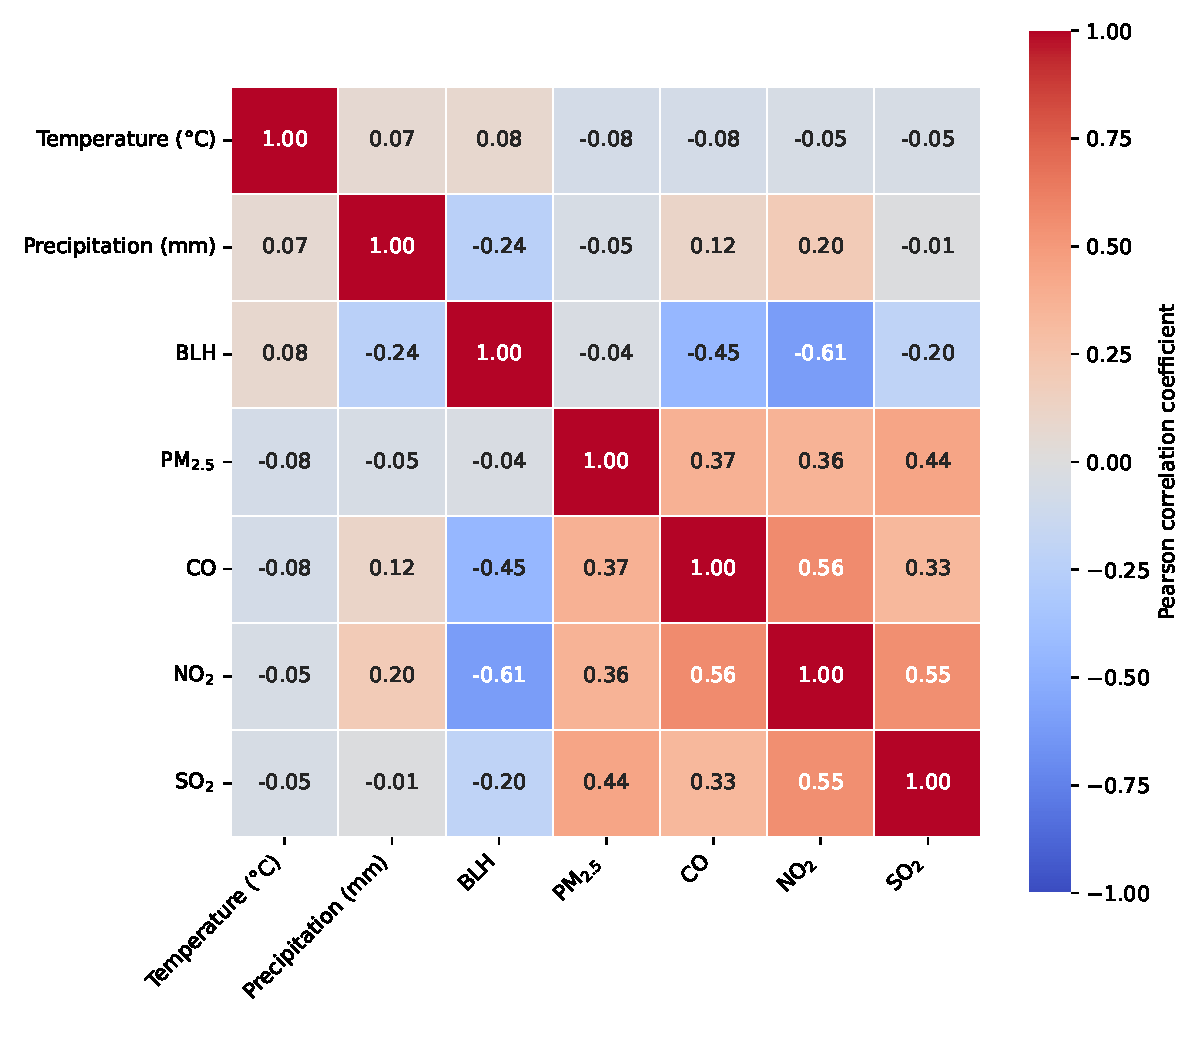
\includegraphics[width=0.8\linewidth]{./picture/correlation_heatmap.pdf}
    \caption{Pearson correlation heatmap between meteorological variables and air pollutants.}
    \label{fig:heatmap}
\end{figure}

\subsection{The proposed method}
This paper proposes an integral analysis of air pollution data and meteorological condition to analyze the air quality in Indonesia. The proposed method is illustrated in Fig 1(ref). The stages of the proposed method are data integration, causal graph generation, and forecasting. The integration process of meteorological data and AQI data use column-based integration. The datasets are time series data with numerical values. The idea of data integration has been used to learn simultaneously from multiple data sensor. The integration data requires not only the same date for each sample but also the same number of samples from all resources. In this paper, the integrated data is a single table containing variables from meteorological data anda AQI data. This data is then used as input for generating a causal graph and forecasting. A causal graph is generated using the PC algorithm. LSTM and GRU are implemented for forecasting.
This paper uses the PC algorithm from $bnlearn$ in the R package. A causal graph is generated in R studio. It also implements LSTM and GRU from TensorFlow Keras. The forecasting is run in Jupyter Notebook for Python. LSTM and GRU models consist of stacked layers with 128 and 64 units, dropout layer and dense layer. LSTM and GRU are run for 50 epochs and they implement the Softmax activation function. This paper uses multivariate forescasting. The experiments use integrated and not integrated data. The letter $i$ and $p$ indicate that the algorithm is implemented for forecasting using integrated data and not integrated data, respectively. A not-integrated data refers to AQI data or a meteorological conditions dataset. An integrated dataset is a dataset containing AQI and meteorological conditions obtained from data integration process. This paper runs multivariate forecasting in 3 different scenarios:

Regional clustering for machine learning analysis - To better capture spatial heterogeneity in pollutant behavior, the Indonesian archipelago is divided into several regional clusters based on geographical and climatic characteristics: Sumatra, Java, Kalimantan, Sulawesi, and Papua–Maluku. These clusters represent distinct environmental and anthropogenic conditions that influence air quality dynamics. For example, Java is characterized by high population density, industrial activities, and transportation emissions, while Sumatra and Kalimantan are frequently affected by biomass burning events associated with land clearing and peatland fires. Sulawesi and the eastern Indonesian region (Papua–Maluku) exhibit different atmospheric circulation patterns and relatively lower anthropogenic emissions. This regional clustering allows the machine learning models to capture localized pollutant behavior, improve predictive performance, and better represent the spatial variability of Air Quality Index (AQI) across the Indonesian archipelago.

Motivation: biomass burning and transboundary pollution - Air quality over Indonesia is strongly influenced by both local emission sources and large-scale atmospheric transport processes. One of the dominant contributors to regional air pollution is biomass burning, particularly from peatland and forest fires occurring in Sumatra and Kalimantan during the dry season. These events release large amounts of atmospheric pollutants such as NO$_2$, CO, SO$_2$, and fine particulate matter (PM$_{2.5}$), which can significantly degrade air quality across the region. In addition to local emissions, transboundary pollution driven by regional atmospheric circulation can transport pollutants across national boundaries within Southeast Asia, affecting neighboring countries and contributing to regional haze events. The complex interaction between emission sources, meteorological conditions, and pollutant transport makes it essential to analyze the behavior of key pollutants using advanced analytical approaches. Integrating ERA5 atmospheric variables, satellite observations, and machine learning techniques provides an effective framework to investigate the spatiotemporal dynamics of air pollution and improve AQI prediction across the Indonesian Maritime Continent.


(Noted) perlu gambar 3. the actual data (A) dan forecasting (B) of AQI

(Noted) Tuliskan semua metodenya disini

\subsection{Meteorological dataset}
ERA5-land (Munoz Sabater, 2019) provides a dataset for land components from ERA5, the fifth-generation climate reanalysis dataset provided by the Copernicus Climate Change Service at the European Centre for Medium-Range Weather Forecasts. Following studies (), we adopted seven meteorological components from the reanalysis dataset: temperature and dew-point temperature at a 2 m height, total evaporation, surface pressure, precipitation and wind components at a 10 m height. We also approximated relative humidity and wind speed using Eq.

ERA5 is the fifth generation ECMWF reanalysis for the global climate and weather for the past 8 decades. Data is available from 1940 onwards. ERA5 provides hourly estimates for a large number of atmospheric, ocean-wave and land-surface quantities. An uncertainty estimate is sampled by an underlying 10-member ensemble at three-hourly intervals. Ensemble mean and spread have been pre-computed for convenience. Such uncertainty estimates are closely related to the information content of the available observing system which has evolved considerably over time. They also indicate flow-dependent sensitive areas. To facilitate many climate applications, monthly-mean averages have been pre-calculated too, though monthly means are not available for the ensemble mean and spread.
ERA5 is a data product (dataset) produced by assimilating many observational sources. It uses satellite observations, but it is not generated by one satellite mission.


Atmospheric variables used in this study were obtained from the ERA5 reanalysis produced by the European Centre for Medium-Range Weather Forecasts through the Copernicus Climate Change Service data archive. The dataset was downloaded using the Copernicus Climate Data Store (CDS) in NetCDF format and subsequently processed using Python-based scientific libraries. The variables analyzed include outgoing longwave radiation (OLR), near-surface air temperature (2 m temperature), and atmospheric trace gases such as nitrogen oxides (NO) and sulfur dioxide (SO$_2$), obtained from the atmospheric composition products associated with the Copernicus reanalysis system. All variables were extracted over the Indonesian domain (6° N–11° S, 95° E–141° E) at a horizontal resolution of 0.25°. The preprocessing procedure involved spatial subsetting of the study region, temporal filtering, unit standardization, and removal of missing values. To reduce short-term variability and emphasize large-scale atmospheric behavior, hourly data were aggregated into daily and monthly means. Spatial averaging was then applied across the regional domain using area-weighted averaging based on latitude to account for grid cell differences. This spatiotemporal aggregation approach enables robust analysis of regional atmospheric variability and long-term climate signals over the Maritime Continent.



\subsection{Study Area}
Indonesia archipelago
Thailand is located at the center of the Indochinese peninsula, has the 10th largest economy in Asia and hosts a population of almost 70 million people (Long and Ascent, 2020). The country is divided into 76 administrative provinces as primary local government units and the capital Bangkok. In this study, considering the meteorological division system in Thailand (), we divided the country into five regions to analyze regional characteristics: north, northeast, central, east and south. Despite the low air quality in Thailand, ground monitoring stations are sparse and mostly concentrated in the central region, which is contains 29 of the 67 stations used in this study. For the remaining regions, 15, 5, 11 and 7 stations are distributed in the north, northeast, east, and south, respectively.

Indonesia is located within the tropical Maritime Continent, a region that plays a crucial role in global atmospheric circulation and climate variability due to its complex land–sea distribution and intense convective activity. The study domain considered in this work covers the Indonesian archipelago approximately between 6° N–11° S latitude and 95° E–141° E longitude, encompassing the major islands of Sumatra, Java, Kalimantan, Sulawesi, Papua, and surrounding smaller island groups. This geographical domain is extracted from the ERA5 reanalysis produced by the European Centre for Medium-Range Weather Forecasts under the Copernicus Climate Change Service. The selected spatial extent captures the key atmospheric processes influencing air pollution variability across Indonesia, including monsoonal circulation, equatorial convection, and regional-scale pollutant transport.

\subsection{Evaluation of general model performance}

\section{Discussion}\label{sec4}
xxxxx.

\section{Conclusion}\label{sec5}
kesimpulan adalah

\backmatter

\bmhead{Declaration and competing interest}
The authors declare that they have no known competing financial interests or personal relationships that could have appeared to influence the work reported in this paper.

\bmhead{Acknowledgements}
This work was supported by UM Internal Grant non-APBN 2026, Indonesia.

\bmhead{Data Availability}
The data that support the findings of this study are available from the corresponding author open reasonable request.

\bmhead{Author Contribution}
The main analysis was led by A.A supervised by H.P. The paper was written by A.A and H.P. and edited by other authors.

\begin{appendices}

\section{Section title of first appendix}\label{secA1}

An appendix contains supplementary information that is not an essential part of the text itself but which may be helpful in providing a more comprehensive understanding of the research problem or it is information that is too cumbersome to be included in the body of the paper.

%%=============================================%%
%% For submissions to Nature Portfolio Journals %%
%% please use the heading ``Extended Data''.   %%
%%=============================================%%

%%=============================================================%%
%% Sample for another appendix section			       %%
%%=============================================================%%

%% \section{Example of another appendix section}\label{secA2}%
%% Appendices may be used for helpful, supporting or essential material that would otherwise 
%% clutter, break up or be distracting to the text. Appendices can consist of sections, figures, 
%% tables and equations etc.

\end{appendices}

\bibliography{atmospheric}% common bib file
%% if required, the content of .bbl file can be included here once bbl is generated
%%\input sn-article.bbl


\end{document}
